% 2011 年广东卷理科第 15 题：过圆 O 外一点 P 作圆的切线 PA 与割线 PBC，
%   C 为圆上一点，BC=5，∠BAC=∠APB。
% 来源 PDF：普通高考/2011/2011广东理.pdf，SHA-256 676f6eb7aaa62d199da64d67e0951301d980eb1e4d82193579afc4a4637ac874。
% 原页：第 1 页（A3 三栏）第 2 栏中部，书页码 663。
% 重绘依据（源为矢量，坐标取自 pdftocairo SVG，真页 pt、原点左上、y 向下）：
%   圆心 O=(629.4,546.8)，半径 40.6pt；P=(534.5,551.7)，A=(610.1,511.1)，B=(589.2,551.7)，
%   C=(611.3,583.2)；切线与圆相切于 A，割线自 P 经 B 穿出圆，水平线终点为圆的右交点 (669.6,551.7)。
%   弦 AB、BC、CA 均为实线，OA 不画。本图取本地坐标 (x,y)=(x_page−520, 600−y_page)，
%   1 单位 = 1 TeX pt，y 向上；拓扑与原页一致，不按原页绝对比例。
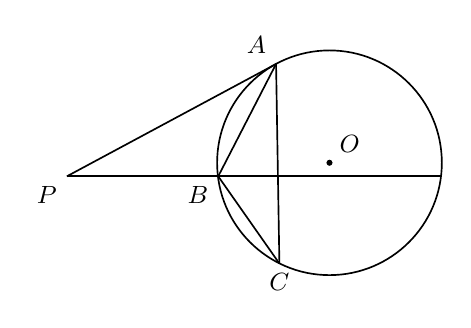
\begin{tikzpicture}[x=1pt, y=1pt, >=stealth, semithick, font=\small]
  \coordinate (O) at (109.4,53.2);
  \coordinate (P) at (14.5,48.3);
  \coordinate (A) at (90.1,88.9);
  \coordinate (B) at (69.2,48.3);
  \coordinate (C) at (91.3,16.8);
  \coordinate (R) at (149.6,48.3);
  % 圆
  \draw (O) circle (40.6pt);
  % 切线 PA 与割线 PBR
  \draw (P) -- (A);
  \draw (P) -- (R);
  % 弦 AB、BC、CA
  \draw (A) -- (B);
  \draw (B) -- (C);
  \draw (A) -- (C);
  % 圆心
  \fill (O) circle (1.1pt);
  % 顶点标注（位置照原页）
  \node[below left] at (P) {$P$};
  \node[above left] at (A) {$A$};
  \node[below left] at (B) {$B$};
  \node[below] at (C) {$C$};
  \node[above right] at (O) {$O$};
\end{tikzpicture}
